% LFM2.5-Audio on AI Glasses -- feasibility report
% Two-column ICML-style layout. Self-contained: no icml*.sty dependency,
% deliberately, so the paper makes no claim of conference publication.
% Build: pdflatex -> pdflatex (twice for refs)

\documentclass[10pt,twocolumn,letterpaper]{article}

\usepackage[letterpaper,left=0.875in,right=0.875in,top=1.0in,bottom=1.0in]{geometry}
\setlength{\columnsep}{0.25in}

\usepackage{times}
\usepackage[T1]{fontenc}
\usepackage[utf8]{inputenc}
\usepackage{microtype}
\usepackage{amsmath}
\usepackage{amssymb}
\usepackage{seqsplit}
\usepackage{textcomp}
\usepackage{booktabs}
\usepackage{multirow}
\usepackage{xcolor}
\usepackage{graphicx}
\usepackage[font=small,labelfont=bf,skip=4pt]{caption}
\usepackage{natbib}
\usepackage{pgfplots}
\usepackage{tikz}
\usetikzlibrary{arrows.meta,positioning,fit,backgrounds}
\pgfplotsset{compat=1.18}
\usepackage[colorlinks=true,linkcolor=black,citecolor=black,urlcolor=blue!60!black]{hyperref}
\usepackage{url}

% --- ICML-ish sectioning ---
\usepackage{titlesec}
\titleformat{\section}{\normalfont\large\bfseries}{\thesection}{0.6em}{}
\titleformat{\subsection}{\normalfont\normalsize\bfseries}{\thesubsection}{0.6em}{}
\titlespacing*{\section}{0pt}{9pt plus 2pt minus 2pt}{4pt}
\titlespacing*{\subsection}{0pt}{7pt plus 2pt minus 2pt}{3pt}

\setlength{\parskip}{0pt}
\setlength{\parindent}{1em}
\renewcommand{\arraystretch}{1.05}

\definecolor{accent}{HTML}{2B4C7E}
\definecolor{warn}{HTML}{9B2C2C}
\definecolor{rulegray}{HTML}{888888}

\newcommand{\pass}{\ensuremath{\checkmark}}
\newcommand{\fail}{\textcolor{warn}{\ensuremath{\times}}}
\newcommand{\taskpass}{\ensuremath{\checkmark}\textsuperscript{\kern-1pt$\dagger$}}
\newcommand{\hash}[1]{\texttt{\scriptsize\seqsplit{#1}}}

\sloppy

\begin{document}

\twocolumn[
\begin{center}
{\LARGE\bfseries LFM2.5-Audio on AI Glasses:\\[2pt]
Feasibility Across Two Hexagon NPU Generations and a Native Phone Deployment\par}
\vspace{10pt}
{\large Ivan A. Novosad\par}
\vspace{4pt}
{\normalsize Public technical report \quad$\cdot$\quad July 16, 2026\par}
\vspace{14pt}
\end{center}

\begin{minipage}{\textwidth}
\begin{center}
\begin{minipage}{0.86\textwidth}
\begin{center}{\bfseries Abstract}\end{center}
\vspace{-4pt}
\small
We evaluate LFM2.5-Audio-1.5B as a speech-to-speech assistant for AI glasses.
With no AR1-class target available, we profile fixed-shape components on two
Qualcomm NPU generations (a QCS8550 proxy and an HTP v81 reference device ---
the target phone's own silicon generation), establish a full-model BF16
reference on an NVIDIA L4, run a Q4 quantization matrix on Apple M2 Metal, and
ship the Q4 bundle as a native Android application on a Snapdragon SM8850
phone. Every neural partition compiles to a strict NPU context with zero CPU
fallback on both generations, 1.46--1.88$\times$ faster on v81; the depth
decoder returns exact tokens and the encoder passes its downstream acceptance
test. The phone demo runs microphone to generated speech end to end with no
host attached, at 0\% WER on the bundled samples and first audio near
800\,ms, and its 1.83\,GiB residency is fully attributed --- chiefly a
556\,MiB CPU weight repack plus fixed compute buffers. Two measured results
set the remaining agenda: FP16 detokenization is numerically unusable on both
NPU generations, so it stays in FP32 on the host; and no tested CPU
configuration clears the 1331\,MiB memory gate, the 0.3\,pp quality rule, and
interactive latency at once. The NPU port is unblocked --- toolchain gate
passed, W8A16 pipeline validated end to end --- and a sub-1B modular pipeline
(Moonshine Base $\rightarrow$ Qwen3-0.6B $\rightarrow$ Pocket TTS) remains the
deployment control.
\end{minipage}
\end{center}
\vspace{12pt}
\end{minipage}
]

% =====================================================================
\section{Introduction}
% =====================================================================

Speech-to-speech assistants on eyewear are constrained less by model quality
than by what a wearable NPU will accept and what its RAM budget will hold.
This report asks a narrow question about one candidate: can
LFM2.5-Audio-1.5B~\citep{lfm25} serve as the integrated baseline for a first
device integration, and what evidence would be needed to call it
glasses-ready?

The answer is a qualified yes on the research track and a not-yet on the
product track. All fixed-shape neural partitions we tested compiled to strict
NPU contexts with zero CPU fallback on the proxy device, and the official BF16
model completed ASR and a persistent two-turn speech interaction on an NVIDIA
L4. The blockers are target-hardware verification, target-QNN resident memory,
a production cache interface, and the output-audio path.

\paragraph{Hardware boundary.}
Every Qualcomm number in this report was measured on QCS8550~(Proxy),
Android~12, Hexagon~v73, through Qualcomm AI Hub~\citep{aihub}. No
AR1/AR1+/5100 target was available. Proxy figures are \emph{placement
evidence}, not AR1 performance, and this qualification applies to every
Qualcomm table and figure below without further repetition.

\paragraph{Contributions.}
\begin{itemize}\itemsep1pt \parskip0pt
\item A strict-placement component profile of LFM2.5-Audio on a Hexagon NPU,
      with per-component latency, peak memory, and numerical acceptance
      (\S\ref{sec:components}).
\item Evidence that full NPU placement and numerical usability are
      independent properties, demonstrated by a fully-placed detokenizer that
      fails on real codes (\S\ref{sec:quality}).
\item A static memory and KV-cache ledger showing why BF16 assets cannot be
      resident in a 2\,GiB budget (\S\ref{sec:memory}).
\item A native-CPU phone deployment whose residency is fully attributed
      (weight repacking, compute geometry, audio-length-scaled encoder
      activations), with a matched on-device 18-utterance diagnostic and a
      negative joint memory--quality--latency verdict (\S\ref{sec:phone}).
\item An HTP v81 transfer matrix on the phone's silicon generation and a
      W8A16 quantization smoke, establishing the NPU port's toolchain path
      and its two open blockers (\S\ref{sec:npu}).
\item A candidate comparison against Whisper, Moonshine, Zipformer, and Piper
      component cards, and the resulting baseline decision
      (\S\ref{sec:candidates}).
\end{itemize}

% =====================================================================
\section{Setup}
% =====================================================================

\subsection{Usage mode}

The product mode is VAD-gated activation followed by a continuous
conversational session. This avoids full-model inference while idle, but it
does not bound active-session context: once a session opens, KV growth is
unbounded until the session manager intervenes. An explicit reset,
summarization, or eviction policy is therefore a requirement, not a
refinement. Figure~\ref{fig:partition} shows the partition we recommend for a
first integration.

\begin{figure}[t]
\centering
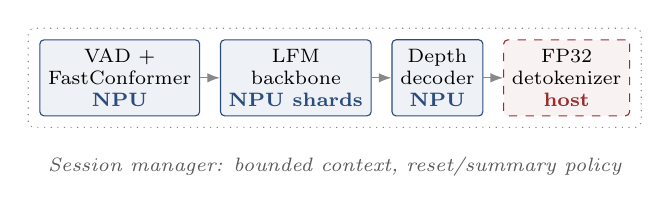
\begin{tikzpicture}[
  font=\scriptsize,
  box/.style={draw=rulegray, rounded corners=1.5pt, align=center,
              minimum height=8.5mm, inner xsep=3pt, fill=black!3},
  npu/.style={box, draw=accent, fill=accent!8},
  host/.style={box, draw=warn, fill=warn!6, dashed},
  ar/.style={-{Latex[length=1.6mm]}, draw=rulegray}
]
\node[npu] (vad) {VAD +\\FastConformer\\\textcolor{accent}{\bfseries NPU}};
\node[npu, right=2.5mm of vad] (bb) {LFM\\backbone\\\textcolor{accent}{\bfseries NPU shards}};
\node[npu, right=2.5mm of bb] (dd) {Depth\\decoder\\\textcolor{accent}{\bfseries NPU}};
\node[host, right=2.5mm of dd] (dt) {FP32\\detokenizer\\\textcolor{warn}{\bfseries host}};
\draw[ar] (vad) -- (bb);
\draw[ar] (bb) -- (dd);
\draw[ar] (dd) -- (dt);
\begin{scope}[on background layer]
\node[draw=rulegray, dotted, rounded corners=2pt, inner sep=4pt,
      fit=(vad)(dt)] (all) {};
\end{scope}
\node[below=2.5mm of all, font=\scriptsize\itshape, text=black!65]
  {Session manager: bounded context, reset/summary policy};
\end{tikzpicture}
\caption{Recommended LFM partition for a first device integration. The host
detokenizer is an architectural recommendation, not a measured on-glasses
result.}
\label{fig:partition}
\end{figure}

\subsection{Evidence classes}

Table~\ref{tab:scope} states what each class of measurement does and does not
establish. The distinction matters throughout: local, proxy, and reference-GPU
evidence are not interchangeable, and none of them is a glasses measurement.

\begin{table}[t]
\centering
\small
\caption{Scope of the experiments. The final row is the part that constrains
every conclusion in this report.}
\label{tab:scope}
\begin{tabular}{@{}p{0.21\columnwidth}p{0.71\columnwidth}@{}}
\toprule
\textbf{Class} & \textbf{Contents} \\
\midrule
Local & Eight official-weight fixed-shape PT2 exports; repeated
Q4\_0/KV-cache matrix on Apple M2 Metal; static memory ledger. \\
\addlinespace[2pt]
Qualcomm proxy & Strict NPU placement, component-only latency and memory,
local-vs-remote numerical comparison. \\
\addlinespace[2pt]
Reference GPU & Full BF16 ASR plus two-turn interleaved text/audio generation
on one NVIDIA L4. \\
\addlinespace[2pt]
Phone (CPU) & Native Android ARM64 Q4 CPU deployment: batch latency, resident
memory attribution, CPU core-seconds, thermal snapshots, matched 18-utterance
diagnostic. Not an NPU path. \\
\addlinespace[2pt]
v81 reference (cloud) & Fixed-shape FP16 transfer and a W8A16 smoke on a
Snapdragon 8 Elite Gen 5 QRD (HTP v81) via AI Hub --- the phone's silicon
generation, not the phone itself. \\
\addlinespace[2pt]
Quality & Downstream encoder sensitivity, exact depth tokens, generated-wave
integrity, small matched ASR diagnostic. \\
\addlinespace[2pt]
\textbf{Not measured} & Full AR1 pipeline, host/NPU transfers, glasses RSS,
power, VAD, microphone-to-speaker latency, an accepted quantized LFM QNN
graph. \\
\bottomrule
\end{tabular}
\end{table}

% =====================================================================
\section{Component placement on the proxy}
\label{sec:components}
% =====================================================================

Every tested strict graph placed fully on the Hexagon NPU
(Table~\ref{tab:components}). Zero operators fell back to CPU in any
partition. Latency spans an order of magnitude, from 1.880\,ms for the
four-frame detokenizer to 25.540\,ms for the depth/RQ decoder, and peak memory
is flat at 87--92\,MiB across all eight graphs.

The two \fail{} rows are the finding. Placement and numerical acceptance are
independent: the detokenizer compiles cleanly, runs fast, and produces audio
that is unusable (\S\ref{sec:quality}). Section~\ref{sec:npu} repeats all
eight graphs on the phone's HTP v81 generation; the pass/fail classes do not
move.

\begin{table}[t]
\centering
\footnotesize
\setlength{\tabcolsep}{3pt}
\caption{Strict-placement component results on QCS8550~(Proxy). NPU/CPU is the
operator split; every graph placed with zero CPU fallback. Numerics:
$\checkmark$ pass, \textcolor{warn}{$\times$} mismatch against the local
golden. $^{\dagger}$Outside the deliberately strict $10^{-3}$ tensor gate
(max abs 0.081) but passes the downstream acceptance test --- 16/17 top-1
decisions preserved, golden in the top-5 throughout (\S\ref{sec:quality}) ---
which is the criterion this report uses.}
\label{tab:components}
\begin{tabular}{@{}lrrrc@{}}
\toprule
\textbf{Component} & \textbf{NPU/CPU} & \textbf{Latency} & \textbf{Peak} & \textbf{Num.} \\
\midrule
FastConformer + adapter & 1215/0 & 4.786\,ms & 87.0\,MiB & \taskpass \\
Conv layer prefill & 36/0 & 2.693\,ms & 92.2\,MiB & \pass \\
Attention layer prefill & 62/0 & 2.444\,ms & 91.5\,MiB & \pass \\
Conv cached decode & 32/0 & 2.695\,ms & 91.9\,MiB & \pass \\
Attention cached decode & 61/0 & 2.452\,ms & 87.0\,MiB & \pass \\
Depth/RQ decoder & 2953/0 & 25.540\,ms & 92.0\,MiB & \pass \\
Detokenizer neural $T{=}4$ & 371/0 & 1.880\,ms & 88.0\,MiB & \fail \\
Detokenizer neural $T{=}8$ & 371/0 & 2.577\,ms & 87.4\,MiB & \fail \\
\bottomrule
\end{tabular}
\end{table}

\begin{figure}[t]
\centering
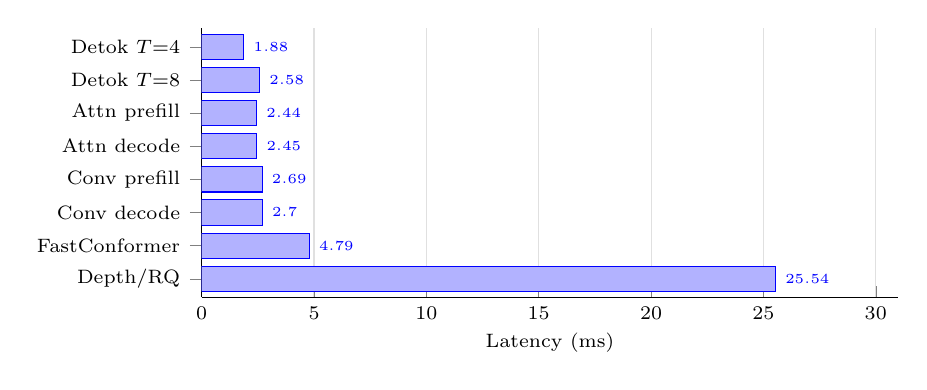
\begin{tikzpicture}
\begin{axis}[
  width=0.86\columnwidth, height=5.0cm,
  xbar, xmin=0, xmax=31,
  bar width=3.2mm,
  font=\scriptsize,
  xlabel={Latency (ms)},
  xlabel style={font=\scriptsize, yshift=2pt},
  symbolic y coords={
    {Detok $T{=}4$},{Detok $T{=}8$},{Attn prefill},{Attn decode},
    {Conv prefill},{Conv decode},{FastConformer},{Depth/RQ}},
  ytick=data,
  y dir=reverse,
  yticklabel style={font=\scriptsize},
  nodes near coords, nodes near coords style={font=\tiny, /pgf/number format/fixed,
    /pgf/number format/precision=2},
  every axis plot/.append style={fill=accent!55, draw=accent},
  axis lines*=left,
  xmajorgrids, grid style={draw=black!12},
  enlarge y limits=0.08,
]
\addplot coordinates {
  (1.880,{Detok $T{=}4$}) (2.444,{Attn prefill}) (2.452,{Attn decode})
  (2.577,{Detok $T{=}8$}) (2.693,{Conv prefill}) (2.695,{Conv decode})
  (4.786,{FastConformer}) (25.540,{Depth/RQ})};
\end{axis}
\end{tikzpicture}
\caption{Per-component latency on the proxy. These values must not be summed:
the components have different shapes, different invocation counts,
different compiled-context overheads, and different transfer boundaries.}
\label{fig:latency}
\end{figure}

% =====================================================================
\section{Full-model reference behavior}
\label{sec:golden}
% =====================================================================

The official BF16 model completed a persistent two-turn speech interaction on
a single NVIDIA L4 (Table~\ref{tab:golden}). Turn~2 is uniformly faster than
turn~1 because the session cache is warm: first text drops from 97.97\,ms to
56.49\,ms and first audio token from 339.67\,ms to 225.87\,ms.

In a separate sequential ASR pass the same checkpoint preprocessed in
0.559\,s, produced its first token at 0.502\,s, and generated 58 tokens in
1.593\,s (36.40 tokens/s). Checkpoint load took 16.104\,s.

The run used 3.034\,GB steady and 6.216\,GB peak CUDA allocation, with
6.388\,GB reserved. These are reference-GPU allocator figures, not mobile RSS
--- \S\ref{sec:phone} supplies the real-device number --- and they are not a
budget for the glasses. The official output detokenizer remained FP32
throughout.

\begin{table}[t]
\centering
\small
\caption{Full-model BF16 golden on one NVIDIA L4. Turn~2 benefits from a warm
session cache.}
\label{tab:golden}
\begin{tabular}{@{}lrr@{}}
\toprule
\textbf{Metric} & \textbf{Turn 1} & \textbf{Turn 2} \\
\midrule
First text & 97.97\,ms & 56.49\,ms \\
First audio token & 339.67\,ms & 225.87\,ms \\
Generated steps/s & 15.74 & 16.35 \\
Decoded waveform & 11.84\,s & 8.96\,s \\
\bottomrule
\end{tabular}
\end{table}

% =====================================================================
\section{Quality}
\label{sec:quality}
% =====================================================================

\subsection{Encoder fidelity}

The encoder path passes its acceptance test. A frozen downstream LFM
sensitivity check on the proxy features preserves 16/17 top-1 decisions ---
the single branch change is \emph{seems} to \emph{looks} --- with the golden
choice in the remote top-five at every step. Feature-space agreement is high
(cosine 0.998424, NRMSE 0.06976, 100\% nearest-frame temporal identity over
ten captured frames) though outside the deliberately strict $10^{-3}$ tensor
gate, and that combination is the point: acceptance is defined at task level,
because the detokenizer below shows that tensor-adjacent metrics can pass
placement and still produce catastrophic output. Every precision change is
therefore re-checked on transcripts, tokens, and task behavior.

\subsection{Detokenizer failure}

The depth/RQ decoder returns exact audio code tokens. The FP16 NPU
detokenizer, given those real generated codes, does not: waveform cosine
0.0052, NRMSE 1.010, and SI-SDR $-45.74$\,dB over the first eight valid
turn-1 frames. The graph still places 371/371 runtime layers on the NPU at
2.564\,ms.

This is the single most consequential result in the report. A component can be
fully accepted by the compiler, run at target speed, and be worthless. The
first device integration should keep the official FP32 detokenizer outside the
FP16 HTP path until a host implementation is measured and accepted.

\subsection{Matched ASR diagnostic}

We transcribed the same 18 LibriSpeech dummy utterances under three
conditions: clean, deterministic 10\,dB white noise, and 5\,dB competing
speech (Table~\ref{tab:wer}, Figure~\ref{fig:wer}). WER is normalized; lower
is better. This is a smoke diagnostic on synthetic noise, not a product
benchmark and not a glasses-microphone benchmark.

LFM is strongest on clean speech (2.86\%) and on 10\,dB white noise (6.43\%).
Under 5\,dB competing speech the ordering inverts: Whisper Small leads at
31.43\% while LFM degrades to 55.71\%. Moonshine Base remains the footprint
challenger, not a demonstrated multi-speaker quality winner.

On the diagnostic itself LFM's mean first-token latency was 101.7\,ms clean,
55.3\,ms under white noise, and 55.6\,ms under competing speech, at real-time
factors of 0.064--0.074 and 3.14\,GB peak allocation. Those are L4 figures and
are not comparable to the Apple MPS runtimes recorded for Moonshine, nor to
any Qualcomm or phone latency in this report.

\begin{table}[t]
\centering
\small
\caption{WER (\%) on the same 18-utterance diagnostic; lower is better. Best
per column in bold.}
\label{tab:wer}
\begin{tabular}{@{}lrrr@{}}
\toprule
\textbf{Model} & \textbf{Clean} & \textbf{White 10\,dB} & \textbf{Compet. 5\,dB} \\
\midrule
LFM2.5 & \textbf{2.86} & \textbf{6.43} & 55.71 \\
Whisper Tiny & 11.43 & 21.67 & 71.90 \\
Whisper Base & 8.81 & 20.71 & 55.00 \\
Whisper Small & 7.14 & 10.71 & \textbf{31.43} \\
Moonshine Base & 8.57 & 14.52 & 64.05 \\
\bottomrule
\end{tabular}
\end{table}

\begin{figure}[t]
\centering
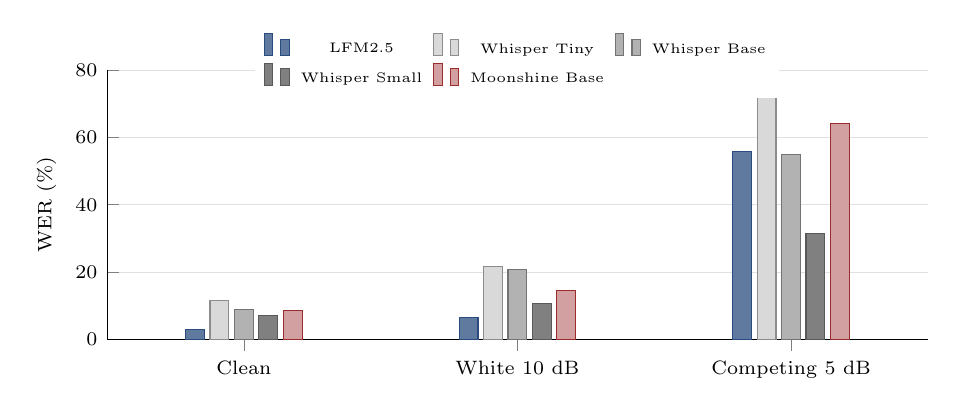
\begin{tikzpicture}
\begin{axis}[
  ybar,
  width=0.99\columnwidth, height=5.0cm,
  font=\scriptsize,
  bar width=2.4mm,
  ymin=0, ymax=80,
  ylabel={WER (\%)},
  ylabel style={font=\scriptsize},
  symbolic x coords={Clean, {White 10 dB}, {Competing 5 dB}},
  xtick=data,
  xticklabel style={font=\scriptsize},
  legend style={at={(0.5,1.16)}, anchor=north, legend columns=3,
                font=\tiny, draw=none, column sep=2pt},
  ymajorgrids, grid style={draw=black!12},
  axis lines*=left,
  enlarge x limits=0.25,
]
\addplot[fill=accent!75, draw=accent] coordinates {(Clean,2.86) ({White 10 dB},6.43) ({Competing 5 dB},55.71)};
\addplot[fill=black!15, draw=black!45] coordinates {(Clean,11.43) ({White 10 dB},21.67) ({Competing 5 dB},71.90)};
\addplot[fill=black!30, draw=black!55] coordinates {(Clean,8.81) ({White 10 dB},20.71) ({Competing 5 dB},55.00)};
\addplot[fill=black!50, draw=black!65] coordinates {(Clean,7.14) ({White 10 dB},10.71) ({Competing 5 dB},31.43)};
\addplot[fill=warn!45, draw=warn] coordinates {(Clean,8.57) ({White 10 dB},14.52) ({Competing 5 dB},64.05)};
\legend{LFM2.5, Whisper Tiny, Whisper Base, Whisper Small, Moonshine Base}
\end{axis}
\end{tikzpicture}
\caption{WER on the 18-utterance diagnostic. The clean-speech ranking does not
survive competing speech.}
\label{fig:wer}
\end{figure}

\subsection{Generated-audio intelligibility}

Retranscribing LFM's own generated audio with Whisper Small gives 0.00\% WER
for turn~1 and 21.43\% WER for turn~2 against LFM's own generated text. The
WAVs are finite, 24\,kHz mono, and unclipped. This is an audio-text
consistency proxy, not a naturalness or MOS score.

% =====================================================================
\section{Memory and context budget}
\label{sec:memory}
% =====================================================================

The pinned BF16 runtime checkpoint set occupies 3.390\,GiB in static files.
The complete local Q4 GGUF bundle occupies 1.001\,GiB --- a 3.39$\times$
smaller package, though across different formats and backends, so it is a
package-to-package comparison and nothing stronger. Static file size is not
process RSS. The consequence stands regardless: the BF16 assets cannot all be
resident inside a 2\,GiB RAM budget.

Active-session growth is dominated by the six attention-layer KV caches
(Table~\ref{tab:kv}); the fixed convolution cache is roughly 0.12\,MiB at
BF16 and never matters. VAD reduces idle work but does not touch this
requirement --- which is why the session policy of \S2.1 is load-bearing.

\begin{table}[t]
\centering
\small
\caption{Ideal KV payload by context length. Tensor-payload estimates only;
actual quantized runtime buffers differ because of scales and alignment.}
\label{tab:kv}
\begin{tabular}{@{}rrr@{}}
\toprule
\textbf{Context positions} & \textbf{FP16 payload} & \textbf{INT8 payload} \\
\midrule
4,096 & 48\,MiB & 24\,MiB \\
8,192 & 96\,MiB & 48\,MiB \\
16,384 & 192\,MiB & 96\,MiB \\
32,768 & 384\,MiB & 192\,MiB \\
\bottomrule
\end{tabular}
\end{table}

% =====================================================================
\section{Local quantization matrix}
\label{sec:q4}
% =====================================================================

The official Q4\_0 GGUF bundle was run 40 times across two official audio
samples with FP16, Q8\_0, and Q4\_0 KV caches plus a flash-attention control.
All 40/40 normalized transcripts match exactly (Table~\ref{tab:q4}). Q4\_0 KV
cuts cache memory from 48.0\,MiB to 13.5\,MiB with no transcript change on
this sample.

This is an Apple M2 Metal sanity check. It is not Qualcomm QNN evidence, not
AR1 evidence, and not a general quality benchmark. The runner reports Metal
fallback hotspots for \texttt{CONV\_2D\_DW}, \texttt{ROLL}, and
\texttt{UNARY} in the audio encoder; those are Metal hotspots, not QNN
CPU-fallback evidence. No quantized LFM QNN graph has yet been profiled on
QCS8550 or on the glasses.

\begin{table*}[t]
\centering
\small
\caption{Local Q4 inference-technique matrix on Apple M2 Metal. Values are
median/p95 over five runs per sample and configuration. CLI model time
excludes model load; wall time in the public data includes process startup and
file-cache effects.}
\label{tab:q4}
\begin{tabular}{@{}llllrrrr@{}}
\toprule
\textbf{KV} & \textbf{Flash} & \textbf{Sample} & \textbf{Exact} & \textbf{KV MiB} &
\textbf{Encode ms} & \textbf{Gen tok/s} & \textbf{Model ms} \\
 & & & & & \textit{med/p95} & \textit{med/p95} & \textit{med/p95} \\
\midrule
FP16 & off & asr & 5/5 & 48.0 & 449.0 / 629.8 & 24.3 / 25.6 & 3425.8 / 3555.5 \\
FP16 & off & question & 5/5 & 48.0 & 140.0 / 298.4 & 29.1 / 57.4 & 816.9 / 1590.3 \\
FP16 & on & asr & 5/5 & 48.0 & 439.0 / 592.4 & 23.2 / 26.4 & 3389.3 / 3855.5 \\
FP16 & on & question & 5/5 & 48.0 & 172.0 / 196.8 & 28.6 / 38.8 & 891.4 / 1096.6 \\
Q4\_0 & on & asr & 5/5 & 13.5 & 413.0 / 476.8 & 25.7 / 26.1 & 3122.0 / 3285.7 \\
Q4\_0 & on & question & 5/5 & 13.5 & 139.0 / 148.8 & 32.6 / 48.6 & 738.1 / 904.6 \\
Q8\_0 & on & asr & 5/5 & 25.5 & 486.0 / 780.4 & 26.5 / 28.1 & 3254.8 / 3780.5 \\
Q8\_0 & on & question & 5/5 & 25.5 & 137.0 / 195.4 & 41.7 / 67.7 & 627.5 / 982.5 \\
\bottomrule
\end{tabular}
\end{table*}

% =====================================================================
\section{Native phone deployment}
\label{sec:phone}
% =====================================================================

\subsection{What this measures}

We packaged the same official Q4 GGUF bundle as a native Android application
and profiled it on a Nubia NX809J (Snapdragon SM8850, Android 16, SDK 36;
14.88\,GiB RAM; eight ARM64 cores in a 6+2 arrangement, six at 3.63\,GHz and
two at 4.74\,GHz). A saved on-device library listing shows an OEM HTP v81
runtime (\texttt{libQnnHtpV81}) that this deployment does not use: the
execution backend is the official Android ARM64 Q4 CPU runner.

The demo is complete on the handset: native microphone capture, streaming
text, and generated speech pass end to end in the embedded UI, and the
application cold-launches and serves a fresh microphone inference with no
computer, cable, or network attached. It is a CPU path --- the NPU port is
\S\ref{sec:npu} --- and it supplies the first measurement of this model
resident on real mobile hardware, the quantity \S\ref{sec:memory} could not
derive from static files.

Two structural properties bound the numbers: complete audio files are
submitted before inference begins (batch timings after utterance completion,
excluding capture and VAD), and reported p95 values at $n \leq 10$ are sample
maxima.

\subsection{Residency: the static-to-resident gap}

Table~\ref{tab:phonemem} is the central result. The Q4 bundle occupies
1.001\,GiB as static files (\S\ref{sec:memory}); the model process resident
set peaks at 1873.4\,MiB, or 1.829\,GiB --- a factor of 1.83. Static size
underpredicts residency by nearly half, which is why the ledger of
\S\ref{sec:memory} is a lower bound and not a budget.

The kernel high-water mark (\texttt{VmHWM}) is 1874.2\,MiB, about 0.8\,MiB
above the sampled peak, so 0.25\,s sampling slightly understates the true
maximum.

\paragraph{Attribution.}
A follow-up batch with a retained runner load log and \texttt{smaps} capture
names the gap. At the original 4096 context, active residency splits into
697.6\,MiB of GGUF-file-backed pages against 1041.2\,MiB of anonymous memory,
and the load log declares the major anonymous allocations
(Table~\ref{tab:attrib}): the largest single item is a 555.75\,MiB CPU weight
\emph{repack} --- a second, kernel-friendly copy of the backbone weights that
coexists with their 652.3\,MiB mmapped originals --- followed by three fixed
compute buffers totaling 458.7\,MiB. The formerly unexplained $\sim$800\,MiB
is therefore repacked weights and compute geometry, not hidden model files.

Context length is a weak lever and audio length a strong one: shrinking
context 4096 to 512 saves only 42.9\,MiB, while moving from the 4.9\,s to the
18.4\,s input raises active residency by roughly 125\,MiB at every context
size (1870.6\,MiB at context 4096 --- consistent with the original run's
1873.4\,MiB peak, which the long-ASR workload set). The longest 29.4\,s
diagnostic utterance drives \texttt{VmHWM} to 1919.3\,MiB with repacking
enabled.

\paragraph{The joint verdict.}
Disabling repacking (\texttt{--no-repack}, context 512) removes 538\,MiB of
active residency and preserves the matched 18-utterance diagnostic within the
0.3\,pp rule on every split --- but peaks at 1365.3\,MiB \texttt{VmHWM} on the
29.4\,s utterance and roughly doubles to triples request latency (single
ordered runs; first audio exceeded 1.2\,s). Configurations pushed to
1302.9--1320.2\,MiB via smaller micro-batches and KV quantization all fail the
competing-speech split by $+0.48$ to $+1.90$\,pp. Stating the gate in explicit
units --- $\leq$1331\,MiB (1.3\,GiB); the stricter decimal reading is
1240\,MiB --- no tested CPU configuration passes memory, quality, and latency
simultaneously. The CPU Q4 deployment is a working demo and research baseline;
it is not an accepted product configuration.

\begin{table}[t]
\centering
\footnotesize
\setlength{\tabcolsep}{4pt}
\caption{Load-log declared allocations behind the anonymous residency
(context 4096). Declared buffers need not be simultaneously resident, so the
column does not sum to \texttt{smaps} RSS; log and \texttt{smaps} agree on the
attribution.}
\label{tab:attrib}
\begin{tabular}{@{}lr@{}}
\toprule
\textbf{Runtime allocation} & \textbf{Declared size} \\
\midrule
Main-model CPU repack & 555.75\,MiB \\
Audio-encoder compute buffer & 195.19\,MiB \\
Main compute buffer & 132.00\,MiB \\
Detokenizer compute buffer & 131.50\,MiB \\
Main KV, context 4096, FP16 & 48.00\,MiB \\
Detokenizer CPU repack & 19.27\,MiB \\
Detokenizer sliding-window KV & 2.25\,MiB \\
\bottomrule
\end{tabular}
\end{table}

\begin{table}[t]
\centering
\footnotesize
\setlength{\tabcolsep}{4pt}
\caption{Peak resident memory on the phone, from \texttt{/proc/<pid>/status}
sampled at a 0.25\,s target interval (172 samples). \texttt{VmRSS} unless
noted. The 1.3\,GB gate is exceeded by the model process alone.}
\label{tab:phonemem}
\begin{tabular}{@{}lrr@{}}
\toprule
\textbf{Process} & \textbf{Peak (MiB)} & \textbf{Peak (bytes)} \\
\midrule
Model (runner) & 1873.4 & 1{,}964{,}384{,}256 \\
\quad kernel \texttt{VmHWM} & 1874.2 & 1{,}965{,}240{,}320 \\
App (UI/service) & 297.0 & 311{,}398{,}400 \\
Combined (sampled) & 2169.1 & 2{,}274{,}426{,}880 \\
\midrule
\textit{Static Q4 bundle} & \textit{1025.0} & \textit{1{,}075{,}000{,}000} \\
\bottomrule
\end{tabular}
\end{table}

\subsection{Latency}

Table~\ref{tab:phonelat} reports the three workloads. Cold start (process
restart, tap to ready) was 823.6/899.3/906.2\,ms over three launches; model
pages remained in the Linux page cache, so this is not a post-reboot cold
load.

The conversational workload reaches first audio at a median 799.7\,ms after
file submission. The gate of \S\ref{sec:gates} asks for first audible PCM
within 500\,ms of VAD close, and no VAD exists in this pipeline, so the two
quantities are not the same measurement and 799.7\,ms should not be read as a
gate result.

\begin{table}[t]
\centering
\footnotesize
\setlength{\tabcolsep}{3pt}
\caption{Phone latency, median/p95 in ms, warm-ups excluded. p95 at these
sample sizes is the maximum observation. ASR workloads emit no audio.}
\label{tab:phonelat}
\begin{tabular}{@{}lrrrr@{}}
\toprule
\textbf{Workload} & \textbf{n} & \textbf{First text} & \textbf{First audio} & \textbf{Total} \\
\midrule
ASR (short) & 10 & 250.9 / 272.4 & --- & 442.5 / 470.9 \\
ASR (long) & 5 & 854.8 / 856.0 & --- & 1554.4 / 1583.5 \\
Chat & 5 & 677.2 / 700.5 & 799.7 / 837.4 & 6786.5 / 6876.9 \\
\bottomrule
\end{tabular}
\end{table}

\subsection{CPU and thermal}

A separate probe attributes 30.62--33.49 core-seconds to the model process
over 3.93--4.26\,s of wall time: an average of 7.86 cores in flight during
generation. The UI/service process rounds to 0.00\,s at the kernel's 100\,Hz
accounting resolution, which reflects rounding rather than idleness; inference
compute lives in the model process. The probe reused a live persistent session
and is therefore not comparable to the fixed-output chat benchmark above.

That the model saturates roughly eight cores is itself the strongest available
evidence that no accelerator is in play: the compute is accounted for on the
CPU.

Thermals moved little across a 52\,s window: CPU maximum 59.0 to
59.4\,\textcelsius{}, GPU 47.8 to 52.9\,\textcelsius{}, NSP 50.9 to
50.5\,\textcelsius{}, skin 28.54 to 35.44\,\textcelsius{}. These are two
snapshots, not a time series, and 52\,s is not a sustained-load test. The
phone was charging throughout, so battery drain was recorded but is not a
valid power measurement and is not reported.

\subsection{Transcript integrity}

All 15 scored ASR runs returned exact normalized transcripts (0.00\% WER)
against the two official demo samples, and all five chat runs produced
byte-identical output (1{,}096{,}320 bytes of float32 PCM, 11.42\,s at
24\,kHz) at temperature 0.

This is the same two-sample check as the Q4 matrix of \S\ref{sec:q4}, extended
from Apple M2 Metal to Android CPU: 40/40 exact there, 15/15 exact here, same
bundle.

The follow-up batch additionally ported a \emph{matched} 18-utterance
diagnostic to the device --- same corpus and deterministic 10\,dB Gaussian and
5\,dB competing-speech variants as \S\ref{sec:quality}, 324 requests with zero
failures. Phone Q4 scores 3.57\,/\,7.14\,/\,54.29\,\% (repack) and
3.57\,/\,6.90\,/\,54.29\,\% (no-repack) against the L4 BF16 reference's
2.86\,/\,6.43\,/\,55.71\,\%. Every gap is within one to two words: at $n{=}18$
($\approx$140 reference words) a single substituted word moves WER by roughly
0.7\,pp, so the instrument is coarser than the 0.3\,pp gate it is asked to
decide. The corpus must be scaled (to $\geq$100 utterances) before any
quantized-WER adjudication.

Byte-count and duration integrity were verified; NaN/Inf validation and
on-device audio-text retranscription were not run.

% =====================================================================
\section{Toward an NPU port}
\label{sec:npu}
% =====================================================================

\subsection{Toolchain gate}

The NPU path required establishing that the phone's Hexagon generation is
reachable at all. It is, twice over: Qualcomm AI Hub exposes the exact silicon
generation --- a Snapdragon 8 Elite Gen 5 QRD (chipset \texttt{sm8850}, HTP
v81) plus the Galaxy S26 family --- and the public QAIRT 2.48.0 community
archive ships the complete v81 target payload for Linux and Windows hosts.
The phone itself carries an OEM QAIRT 2.37.0 v81 runtime. macOS is not a
supported QAIRT host, so local compilation requires an ARM64 Linux
environment; AI Hub covers the interim. Results below come from the QRD, a
reference device of the phone's silicon generation.

\subsection{FP16 transfer to HTP v81}

All eight fixed-shape graphs were re-submitted, unmodified, as strict FP16
context binaries for v81, and every one places fully on the NPU at
1.46--1.88$\times$ lower component latency than v73
(Table~\ref{tab:v81}). The depth/RQ decoder keeps exact tokens after one
boundary correction (\texttt{--truncate\_64bit\_io}; int32 at the QNN
boundary, exactly equal to the int64 goldens). Peaks sit at
117.5--118.0\,MiB, a near-uniform $+25$--$31$\,MiB over v73 regardless of
component size --- consistent with a runtime-baseline change, not per-model
growth.

The stable result matters most: the numerical classes are identical across
the silicon generation and the toolchain revision. Backbone and depth pass on
both; the encoder reproduces v73's accepted signature (cosine 0.998423 versus
0.998424); both detokenizer probes remain unusable on both (v81 angle cosine
0.26--0.28). The partition of Figure~\ref{fig:partition} is a property of the
model, not of v73 or an old compiler --- and FP32 host detokenization is now a
design decision validated across a hardware generation.

\begin{table*}[t]
\centering
\small
\caption{FP16 transfer matrix, v73 (QCS8550 proxy) versus v81 (8 Elite Gen 5
QRD). Placement is identical and fully on-NPU on both generations. Caveat:
v73 numbers were compiled by the AI Hub toolchain current at their submission
date; v81 numbers use the current toolchain. Differences reflect silicon
generation and toolchain version jointly; neither is isolated.
$^{\dagger}$Outside the strict $10^{-3}$ tensor gate; the identical v73
feature signature passed the downstream acceptance test (\S\ref{sec:quality});
the downstream check on v81 features is queued.}
\label{tab:v81}
\begin{tabular}{@{}lrrrrrl@{}}
\toprule
\textbf{Component} & \textbf{Layers} & \textbf{v73} & \textbf{v81} & \textbf{Speedup} & \textbf{Peak v81} & \textbf{Numerics (both gens)} \\
\midrule
FastConformer + adapter & 1215 & 4.786\,ms & 3.185\,ms & 1.50$\times$ & 117.6\,MiB & task pass$^{\dagger}$ \\
Backbone conv prefill & 36 & 2.693\,ms & 1.833\,ms & 1.47$\times$ & 117.7\,MiB & pass \\
Backbone attention prefill & 62 & 2.444\,ms & 1.667\,ms & 1.47$\times$ & 117.7\,MiB & pass \\
Backbone conv cached decode & 32 & 2.695\,ms & 1.831\,ms & 1.47$\times$ & 117.5\,MiB & pass \\
Backbone attention cached decode & 61 & 2.452\,ms & 1.673\,ms & 1.47$\times$ & 117.8\,MiB & pass \\
Depth/RQ decoder & 2953 & 25.540\,ms & 16.778\,ms & 1.52$\times$ & 117.8\,MiB & tokens exact; embedding pass \\
Detokenizer $T{=}4$ & 371 & 1.880\,ms & 1.284\,ms & 1.46$\times$ & 117.9\,MiB & mismatch \\
Detokenizer $T{=}8$ & 371 & 2.577\,ms & 1.372\,ms & 1.88$\times$ & 118.0\,MiB & mismatch \\
\bottomrule
\end{tabular}
\end{table*}

\subsection{Quantization smoke (W8A16)}

A first quantization pass validated mechanics, not quality. The depth/RQ
decoder --- chosen because its acceptance is binary --- was blocked before
compilation: seven \texttt{to\_logits} weights are tied, consumed by both a
\texttt{Gemm} (output projection) and a \texttt{Gather} (embedding lookup),
and the quantizer requires each initializer duplicated per consumer. This is a
mechanical graph-preparation fix, with one watch item: duplication quantizes
seven large tensors twice, so the resulting binary size needs checking.

The conv-prefill fallback completed the full pipeline --- quantize, strict v81
compile, profile, inference --- with full NPU placement, a 64.6\,MiB binary
(49.6\% of FP16), and 0.977\,ms latency (1.88$\times$ faster than its
current-toolchain FP16 comparator). Its output sits outside the FP16
transfer tolerance (max abs error 0.0230, cosine 0.9999955) --- a number that
is currently uninformative in either direction: calibration used a single
example (the 80-sample real-embedding set is captured and awaits export
approval), and quantized graphs are accepted on transcripts and tokens
(\S\ref{sec:quality}), not tensor distance. The calibrated downstream run is
queued and will decide it.

\subsection{Per-step arithmetic and the next gate}

A deliberately naive floor: assuming the LFM2 backbone layout of ten
convolution and six attention blocks (six is fixed by the KV-cache accounting
of \S\ref{sec:memory}), one generation step on v81 costs
$10 \times 1.831 + 6 \times 1.673 + 16.778 \approx 45$\,ms of pure component
time --- about 22 steps/s, with the depth decoder alone taking 37\% of the
budget. The no-summing rule of Figure~\ref{fig:latency} applies in full: this
arithmetic excludes every transfer, graph switch, and cache-management cost,
which on an explicit-cache-I/O design is exactly where the budget is most
likely to go. It motivates, and does not replace, an on-device step-rate
microbenchmark with QNN registered shared buffers as the next gate before any
application work.

% =====================================================================
\section{Comparators and candidate selection}
\label{sec:candidates}
% =====================================================================

\subsection{Qualcomm speech component cards}

Table~\ref{tab:comparators} reports full-NPU proxy scorecards from
\texttt{qai-hub-models} 0.57.3 for the alternative pipeline components. These
are fixed component invocations, not end-to-end pipeline latency.

Whisper Small W8A16 is instructive: quantization makes the encoder
2.89$\times$ slower while making the decoder roughly 35\% faster. Quantization
must therefore be profiled stage by stage; a single whole-model figure would
have hidden both effects.

\begin{table*}[t]
\centering
\small
\caption{Qualcomm proxy component cards for comparator models
(\texttt{qai-hub-models} 0.57.3). Fixed component invocations, not end-to-end
pipeline latency.}
\label{tab:comparators}
\begin{tabular}{@{}llll@{}}
\toprule
\textbf{Model} & \textbf{Encoder/main} & \textbf{Recurrent} & \textbf{Use} \\
\midrule
Zipformer & 8.895\,ms / 0.71\,s chunk & 0.075\,ms dec.; 0.187\,ms joiner & Streaming fallback \\
\addlinespace[1pt]
Whisper Tiny & 25.307\,ms & 2.459\,ms dec. & Small control \\
\addlinespace[1pt]
Whisper Base & 47.978\,ms & 4.202\,ms dec. & Middle control \\
\addlinespace[1pt]
Whisper Small FP16 & 130.318\,ms & 12.074\,ms dec. & Overlap-robust control \\
\addlinespace[1pt]
Whisper Small W8A16 & 376.895\,ms & 7.856\,ms dec. & Memory tradeoff \\
\addlinespace[1pt]
Piper TTS & 30.344\,ms enc.; 15.189\,ms flow & 3.018\,ms dec. & Audio fallback \\
\bottomrule
\end{tabular}
\end{table*}

\subsection{Decision}

Table~\ref{tab:decision} records the candidate outcome. LFM2.5-Audio continues
as the integrated research baseline under the gates of \S\ref{sec:gates}.
Moonshine Base $\rightarrow$ Qwen3-0.6B $\rightarrow$ Pocket
TTS~\citep{moonshine,qwen3,pocket} is the recommended next challenger: it
creates the most weight-footprint headroom while keeping the text model on a
known Qualcomm path. It still needs export, quality, and host-TTS
measurements before it can replace LFM.

LLaMA-Omni2-0.5B~\citep{llamaomni2} is excluded on evidence rather than
principle: the size label refers to the language backbone, while the
checkpoint alone is 3.857\,GB in BF16.

\begin{table}[t]
\centering
\footnotesize
\setlength{\tabcolsep}{2.5pt}
\caption{Candidate decisions. Footprint figures come from different sources
and are not directly comparable.}
\label{tab:decision}
\begin{tabular}{@{}p{0.29\columnwidth}p{0.33\columnwidth}p{0.24\columnwidth}@{}}
\toprule
\textbf{Candidate} & \textbf{Footprint view} & \textbf{Decision} \\
\midrule
LFM2.5-Audio & Q4 bundle 1.001\,GiB locally & Continue with gates \\
\addlinespace[2pt]
Moonshine + Qwen3-0.6B + Pocket & Est.\ 0.55--0.66\,GB weights & Profile next \\
\addlinespace[2pt]
Zipformer + Qwen3-0.6B + Piper & \textasciitilde0.84\,GB from component cards & Demo insurance \\
\addlinespace[2pt]
Mini-Omni~\citep{miniomni} & \textasciitilde976M total est. & Later control \\
\addlinespace[2pt]
LLaMA-Omni2-0.5B & Checkpoint alone 3.857\,GB BF16 & Exclude \\
\bottomrule
\end{tabular}
\end{table}

% =====================================================================
\section{Gates and next steps}
\label{sec:gates}
% =====================================================================

\subsection{Demo acceptance gates}

Table~\ref{tab:gates} lists provisional thresholds for a demo, alongside what
the CPU phone run of \S\ref{sec:phone} does and does not say about each. The
thresholds are provisional in a specific sense: the memory gate is a guess
until app-available RAM on the real device is confirmed, and should be revised
the moment it is.

The memory gate is now stated in explicit units --- $\leq$1331\,MiB
(1.3\,GiB), with the stricter decimal reading 1.3\,GB $=$ 1240\,MiB noted for
reference --- and it is missed: the best quality-preserving configuration
peaks at 1365.3\,MiB, and every configuration under the threshold fails the
competing-speech quality split (\S\ref{sec:phone}). The frontier is three-way:
memory, quality, and latency trade against each other and no tested CPU
configuration holds all three. Three of the remaining gates are not merely
unmeasured but \emph{not exercisable} on a CPU deployment: there are no NPU
shards for a placement gate to inspect, no VAD for a responsiveness gate to
trigger from, and no multi-turn workload for a retention gate to score. This
is a property of the deployment, not an oversight in it.

\begin{table*}[t]
\centering
\footnotesize
\setlength{\tabcolsep}{5pt}
\caption{Provisional demo acceptance gates and their status after the CPU
phone run (\S\ref{sec:phone}). The phone is not the glasses and not an NPU
path; ``not exercisable'' means the deployment contains nothing the gate could
measure.}
\label{tab:gates}
\begin{tabular}{@{}p{0.14\textwidth}p{0.36\textwidth}p{0.40\textwidth}@{}}
\toprule
\textbf{Gate} & \textbf{Provisional threshold} & \textbf{Phone (CPU) status} \\
\midrule
Memory & Model-process peak $\leq$ 1331\,MiB (1.3\,GiB) & \textcolor{warn}{\textbf{Missed}}: best quality-preserving config 1365.3\,MiB \\
\addlinespace[2pt]
Placement & No unsupported main-backbone op; no undeclared CPU fallback & Not exercisable: no NPU shards in this path \\
\addlinespace[2pt]
ASR quality & Quantized WER increase $\leq$ 0.3\,pp per split & Screened: matched $n{=}18$ set; resolution ($\sim$0.7\,pp/word) coarser than the gate \\
\addlinespace[2pt]
Responsiveness & First audible PCM $\leq$ 500\,ms after VAD close & Not exercisable: no VAD; 799.7\,ms post-submission \\
\addlinespace[2pt]
Context & Two-turn retention within five points of BF16 golden & Not exercisable: all workloads single-turn \\
\addlinespace[2pt]
Audio & No NaN/Inf, truncation, or audio-text regression & Partial: byte/duration integrity only \\
\bottomrule
\end{tabular}
\end{table*}

\subsection{Next steps}

\begin{enumerate}\itemsep2pt \parskip0pt
\item Unblock depth quantization: duplicate the seven tied
      \texttt{to\_logits} initializers, calibrate with the captured 80-sample
      real-embedding set, and accept on exact tokens --- then W4A16 the
      backbone, since W8A16 alone roughly doubles the Q4 weight footprint and
      exceeds the memory gate on weights.
\item Run the on-device step-rate microbenchmark with QNN registered shared
      buffers: prefill plus $N$ cached decode steps plus depth, measuring
      transfer overhead against the $\sim$45\,ms naive floor of
      \S\ref{sec:npu}, before any application integration.
\item Recover repack memory without repack latency on the CPU baseline:
      selective repacking, releasing mmapped originals of repacked tensors, or
      staged encoder/detokenizer loading (the encoder's fixed 195\,MiB buffer
      and length-scaled activations are the peak drivers).
\item Scale the matched diagnostic to $\geq$100 utterances so the 0.3\,pp
      quality gate becomes decidable; the current $n{=}18$ resolution is
      $\sim$0.7\,pp per word.
\item Measure the official FP32 detokenizer on the intended host path; the
      FP16 HTP route is closed on both tested silicon generations.
\item Run the unplugged 30-minute power and thermal series (the batch's
      cached 99.6\,\textcelsius{} CPU readings after 324 requests are warning
      evidence, not a sustained result).
\item Profile the modular challenger in parallel --- Qwen3-0.6B, then
      Moonshine Base, then Pocket TTS --- with Zipformer and Piper as swaps.
\item Confirm the physical glasses SoC, app-available RAM, QNN/Voice AI SDK
      version, and deployment interface; repeat the accepted configuration
      there.
\end{enumerate}

% =====================================================================
\section{Limitations}
\label{sec:limits}
% =====================================================================

The proxy is not the target. QCS8550 latency is not AR1 latency, and no
AR1/AR1+/5100 device was available for any measurement in this report.

Component latency and memory cannot be summed into an end-to-end figure. The
components have different shapes, invocation counts, compiled-context
overheads, and transfer boundaries, and Figure~\ref{fig:latency} should not be
read as a budget.

Backbone evidence is representative rather than one full compiled network. The
ASR diagnostic uses 18 utterances and synthetic noise, and is not a glasses
microphone benchmark. Host FP32 detokenizer viability is proposed, not
measured on target. The Q4 matrix uses two official samples on Apple M2 Metal
and establishes neither general quality, nor Qualcomm placement, nor glasses
memory.

The phone deployment is a CPU path on a flagship handset. It is not an NPU
result, not AR1, and not the glasses, and its residency figure transfers to
the glasses only as a lower bound on what a Q4 CPU runner costs. Device
identity is now on record (14.88\,GiB RAM, ARM64, 6+2 cores), and a saved
library listing shows an unused OEM HTP v81 runtime, so the CPU-only claim
rests on positive evidence. Phone thermals remain snapshots --- the batch's
post-run cached 99.6\,\textcelsius{} CPU readings are warning evidence, not a
sustained-load profile --- and the phone was charging, so no power figure is
reported. Phone p95 values at $n \leq 10$ are sample maxima; resident-memory
peaks are sampled at 0.25\,s; and the no-repack latency comparison is single
ordered runs, not a distribution.

The v81 results come from a cloud reference device of the phone's silicon
generation, profiled through AI Hub: isolated fixed-shape component calls with
no transfers, cache management, or end-to-end path, on a QRD rather than
retail hardware, and with silicon and toolchain versions jointly confounded
against the v73 baseline. The W8A16 smoke is a mechanics result only: its
calibration was a single example and its tensor-tolerance verdict is not the
prescribed acceptance test for quantized graphs, so no quantization-quality
conclusion is drawn from it.

Finally, licensing is not settled: the LFM Open License v1.0 contains a
commercial-use revenue threshold, and the candidate components carry separate
attribution and license terms.

\bibliographystyle{plainnat}
\begin{thebibliography}{99}
\footnotesize
\setlength{\itemsep}{0pt}
\setlength{\parskip}{0pt}

\bibitem[Liquid AI(2026a)]{lfm25}
Liquid AI.
\newblock LFM2.5-Audio-1.5B model card.
\newblock \url{https://huggingface.co/LiquidAI/LFM2.5-Audio-1.5B}.

\bibitem[Liquid AI(2026b)]{liquidaudio}
Liquid AI.
\newblock liquid-audio source repository.
\newblock \url{https://github.com/Liquid4All/liquid-audio}.

\bibitem[Qualcomm(2026)]{aihub}
Qualcomm.
\newblock AI Hub model catalog.
\newblock \url{https://aihub.qualcomm.com/models/}.

\bibitem[Qualcomm Zipformer(2026)]{zipformer}
Qualcomm.
\newblock Zipformer model card.
\newblock \url{https://aihub.qualcomm.com/models/zipformer}.

\bibitem[Qualcomm Whisper(2026)]{whispersmall}
Qualcomm.
\newblock Whisper Small model card.
\newblock \url{https://aihub.qualcomm.com/models/whisper_small}.

\bibitem[Qualcomm Piper(2026)]{piper}
Qualcomm.
\newblock PiperTTS English model card.
\newblock \url{https://aihub.qualcomm.com/models/pipertts_en}.

\bibitem[Useful Sensors(2024)]{moonshine}
Useful Sensors.
\newblock Moonshine Base model card.
\newblock \url{https://huggingface.co/UsefulSensors/moonshine-base}.
\newblock arXiv:2410.15608.

\bibitem[Qwen Team(2025)]{qwen3}
Qwen Team.
\newblock Qwen3-0.6B model card.
\newblock \url{https://huggingface.co/Qwen/Qwen3-0.6B}.
\newblock Qualcomm card: \url{https://aihub.qualcomm.com/models/qwen3_0_6b}.

\bibitem[Kyutai Labs(2025)]{pocket}
Kyutai Labs.
\newblock Pocket TTS.
\newblock \url{https://github.com/kyutai-labs/pocket-tts}.

\bibitem[Xie \& Wu(2024)]{miniomni}
Z.~Xie and C.~Wu.
\newblock Mini-Omni: Language models can hear, talk while thinking in streaming.
\newblock arXiv:2408.16725, 2024.

\bibitem[Fang et al.(2025)]{llamaomni2}
Q.~Fang et al.
\newblock LLaMA-Omni2: LLM-based real-time spoken chatbot with autoregressive
streaming speech synthesis.
\newblock arXiv:2505.02625, 2025.

\end{thebibliography}

% =====================================================================
\appendix
\section{Reproducibility}
\label{sec:repro}
% =====================================================================

\begin{table*}[t]
\centering
\footnotesize
\caption{Pinned revisions and environments. Hashes are unbroken for
copy-paste.}
\label{tab:repro}
\begin{tabular}{@{}p{0.16\textwidth}p{0.78\textwidth}@{}}
\toprule
\textbf{Item} & \textbf{Pinned value} \\
\midrule
LFM model revision & \texttt{c362a0625dfe45aa588dce5f0ada28a7e5707628} \\
\addlinespace[2pt]
Q4 GGUF / runner & \texttt{7d525f883a077e20afb782f2ff618edcae0e39e4}; build 7641 (\texttt{68d8edf2}); Apple M2 Metal \\
\addlinespace[2pt]
Liquid Audio source & \texttt{19e65845923a7f136442c95137884ec61eb386aa} \\
\addlinespace[2pt]
Qualcomm proxy & QCS8550 (Proxy), Android 12, Hexagon v73, QNN HTP FP16 \\
\addlinespace[2pt]
Comparator catalog & \texttt{qai-hub-models} 0.57.3; QAIRT 2.45.0 scorecards \\
\addlinespace[2pt]
Full-model golden & PyTorch 2.8.0, Transformers 4.56.1, NVIDIA L4 BF16; seed 20260715 \\
\addlinespace[2pt]
Phone target & Nubia NX809J, Snapdragon SM8850, Android 16 (SDK 36); official Android ARM64 Q4 CPU runner \\
\addlinespace[2pt]
Phone run & \texttt{20260716t120118z}; 172 resource samples at 0.25\,s target interval; 100\,Hz CPU accounting \\
\addlinespace[2pt]
Phone batch & \texttt{experiment\_batch\_20260717}; attribution, sweeps, and matched diagnostic (324 requests) \\
\addlinespace[2pt]
NPU toolchain & AI Hub target Snapdragon 8 Elite Gen 5 QRD (\texttt{sm8850}, HTP v81); \texttt{qai-hub} 0.52.0; public QAIRT 2.48.0; phone OEM QNN runtime 2.37.0 \\
\addlinespace[2pt]
Depth calibration & 80 embeddings, audio frames 0--79, generation steps 6--120 of the pinned turn \\
 & NPZ SHA-256 \texttt{2e3e4e282385339c1f09574107a64cde31457b40c80c55ea064a2911bb8b35e2} \\
\bottomrule
\end{tabular}
\end{table*}

\paragraph{Phone-run provenance.}
The published \texttt{REPORT.md} is the profiler's generated output plus a
hand-inserted CPU-probe summary section sourced from \texttt{cpu\_probe.json};
\texttt{profile.json} was likewise augmented with that probe summary, which the
profiler does not itself emit. Both edits are numerically faithful: every
published value was verified by regenerating the report from the raw JSON and
diffing, and the \texttt{runs.csv} aggregates recompute to the published
medians and p95 values exactly. The run directory was imported into the
repository on the following day, so file modification times postdate the run
stamp. The profiler's \texttt{lfm-server.log} was excluded from the published
directory; the directory is otherwise what the script produces. The v81
transfer and W8A16 reports were likewise hand-written from script-generated
raw archives with all AI Hub job identifiers retained, and later runs keep
their server logs. Archived JSON evidence had absolute local path strings
redacted post-capture; measured values are unchanged.

\end{document}
